\clearpage 

  \begin{center} 
 
\includegraphics[width=\textwidth ]{www/h1.png} 

   
 
\includegraphics[width=\textwidth ]{www/h2_resumo.png} 
 \end{center} 
 \vspace{-1.5cm} 
  \begin{flushleft} 

              \begin{tabular}{ c c c c c c }
  \hspace{0.5cm} {\Large  364319 } &  \hspace{1.0cm} {\Large  232370 } &  \hspace{1.0cm} {\Large  205033 } &  \hspace{1.0cm} {\Large  1793.194 } &  \hspace{1.1cm} {\Large  382 } &  \hspace{1.8cm} {\Large  184 } \\ 
  \end{tabular}

                 \end{flushleft}
\begin{table}[!h]

\caption{Resumo de informacoes dos casos de Dengue, Dengue com Sinais de Alarme (D.S.A) e Dengue Grave (D.G) referente ao periodo de 28/07/2019 a 16/07/2020}
\centering
\begin{tabular}[t]{lc}
\toprule
  & Periodo  28/07/2019  a  16/07/2020\\
\midrule
Municipios com Notificacao & 382\\
Municipios com casos confirmados (Dengue, D.S.A, D.G) & 349\\
Municipios Autoctones & 326\\
Regionais com casos confirmados & 22\\
Total de Casos Notificados & 364319\\
\addlinespace
Total de Casos Confirmados (Dengue, D.S.A, D.G) & 232370\\
Dengue Sinais de Alarme & 2867\\
Dengue Grave & 279\\
Total de Casos Autoctones & 205033\\
Municipios em Epidemia & 254\\
\addlinespace
Municipios em Alerta & 31\\
Municipios com indice baixo & 64\\
Municipios sem casos & 50\\
Número de Obitos & 184\\
\bottomrule
\end{tabular}
\end{table}\clearpage 

  \begin{center} 
 
\includegraphics[width=\textwidth ]{www/h2.png} 

 \end{center} 

Definicao: Descreve de forma resumida a distribuicao de frequencias da doenca para o periodo de um ano, baseado no 
         comportamento observado da doenca durante varios anos previos (dez anos, excluindo-se os anos epidemico) e em sequencia,
         em determinada populacao. Auxilia na determinacao de situacoes de alerta epidemico e previsao de epidemias, atraves da 
         sobreposicao da curva epidemica do periodo de interesse (frequencia observada do ano atual) ao canal endemico (frequencia esperada). 
   
 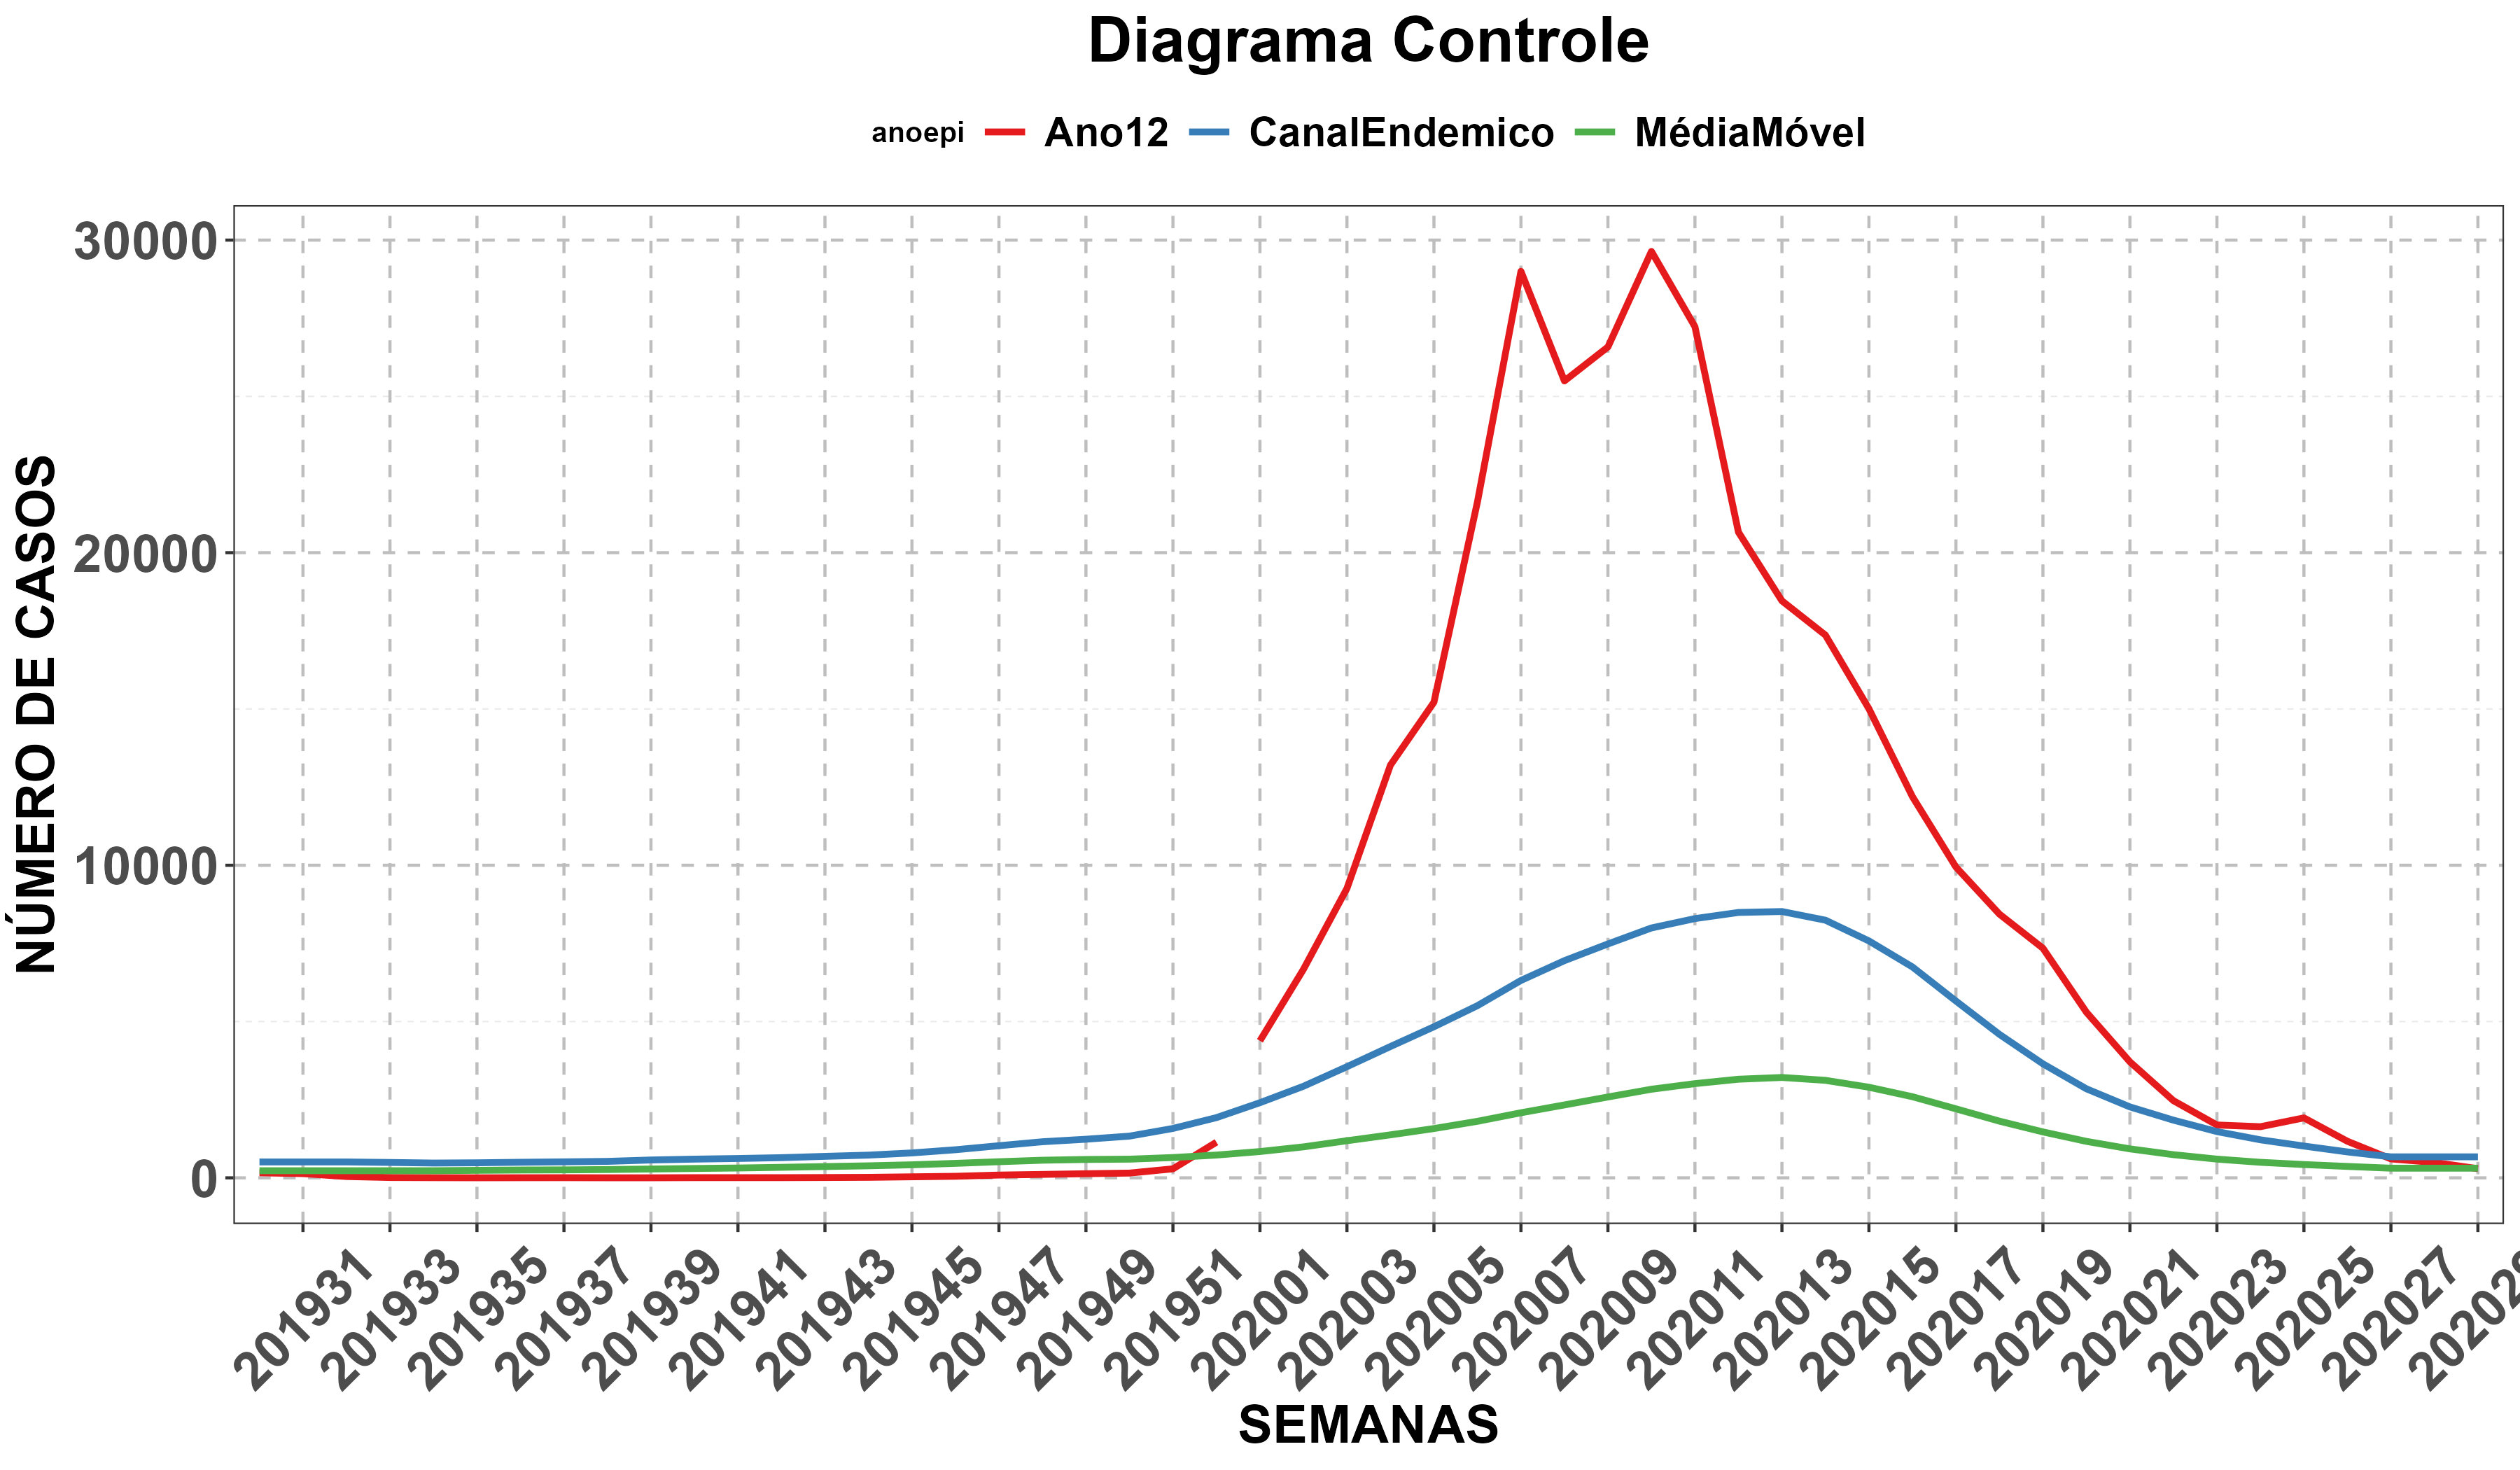
\includegraphics[width=16cm]{diagramacontrole.png} 
  
 \clearpage 

 
\includegraphics[width=\textwidth ]{www/h3.png}  

 
 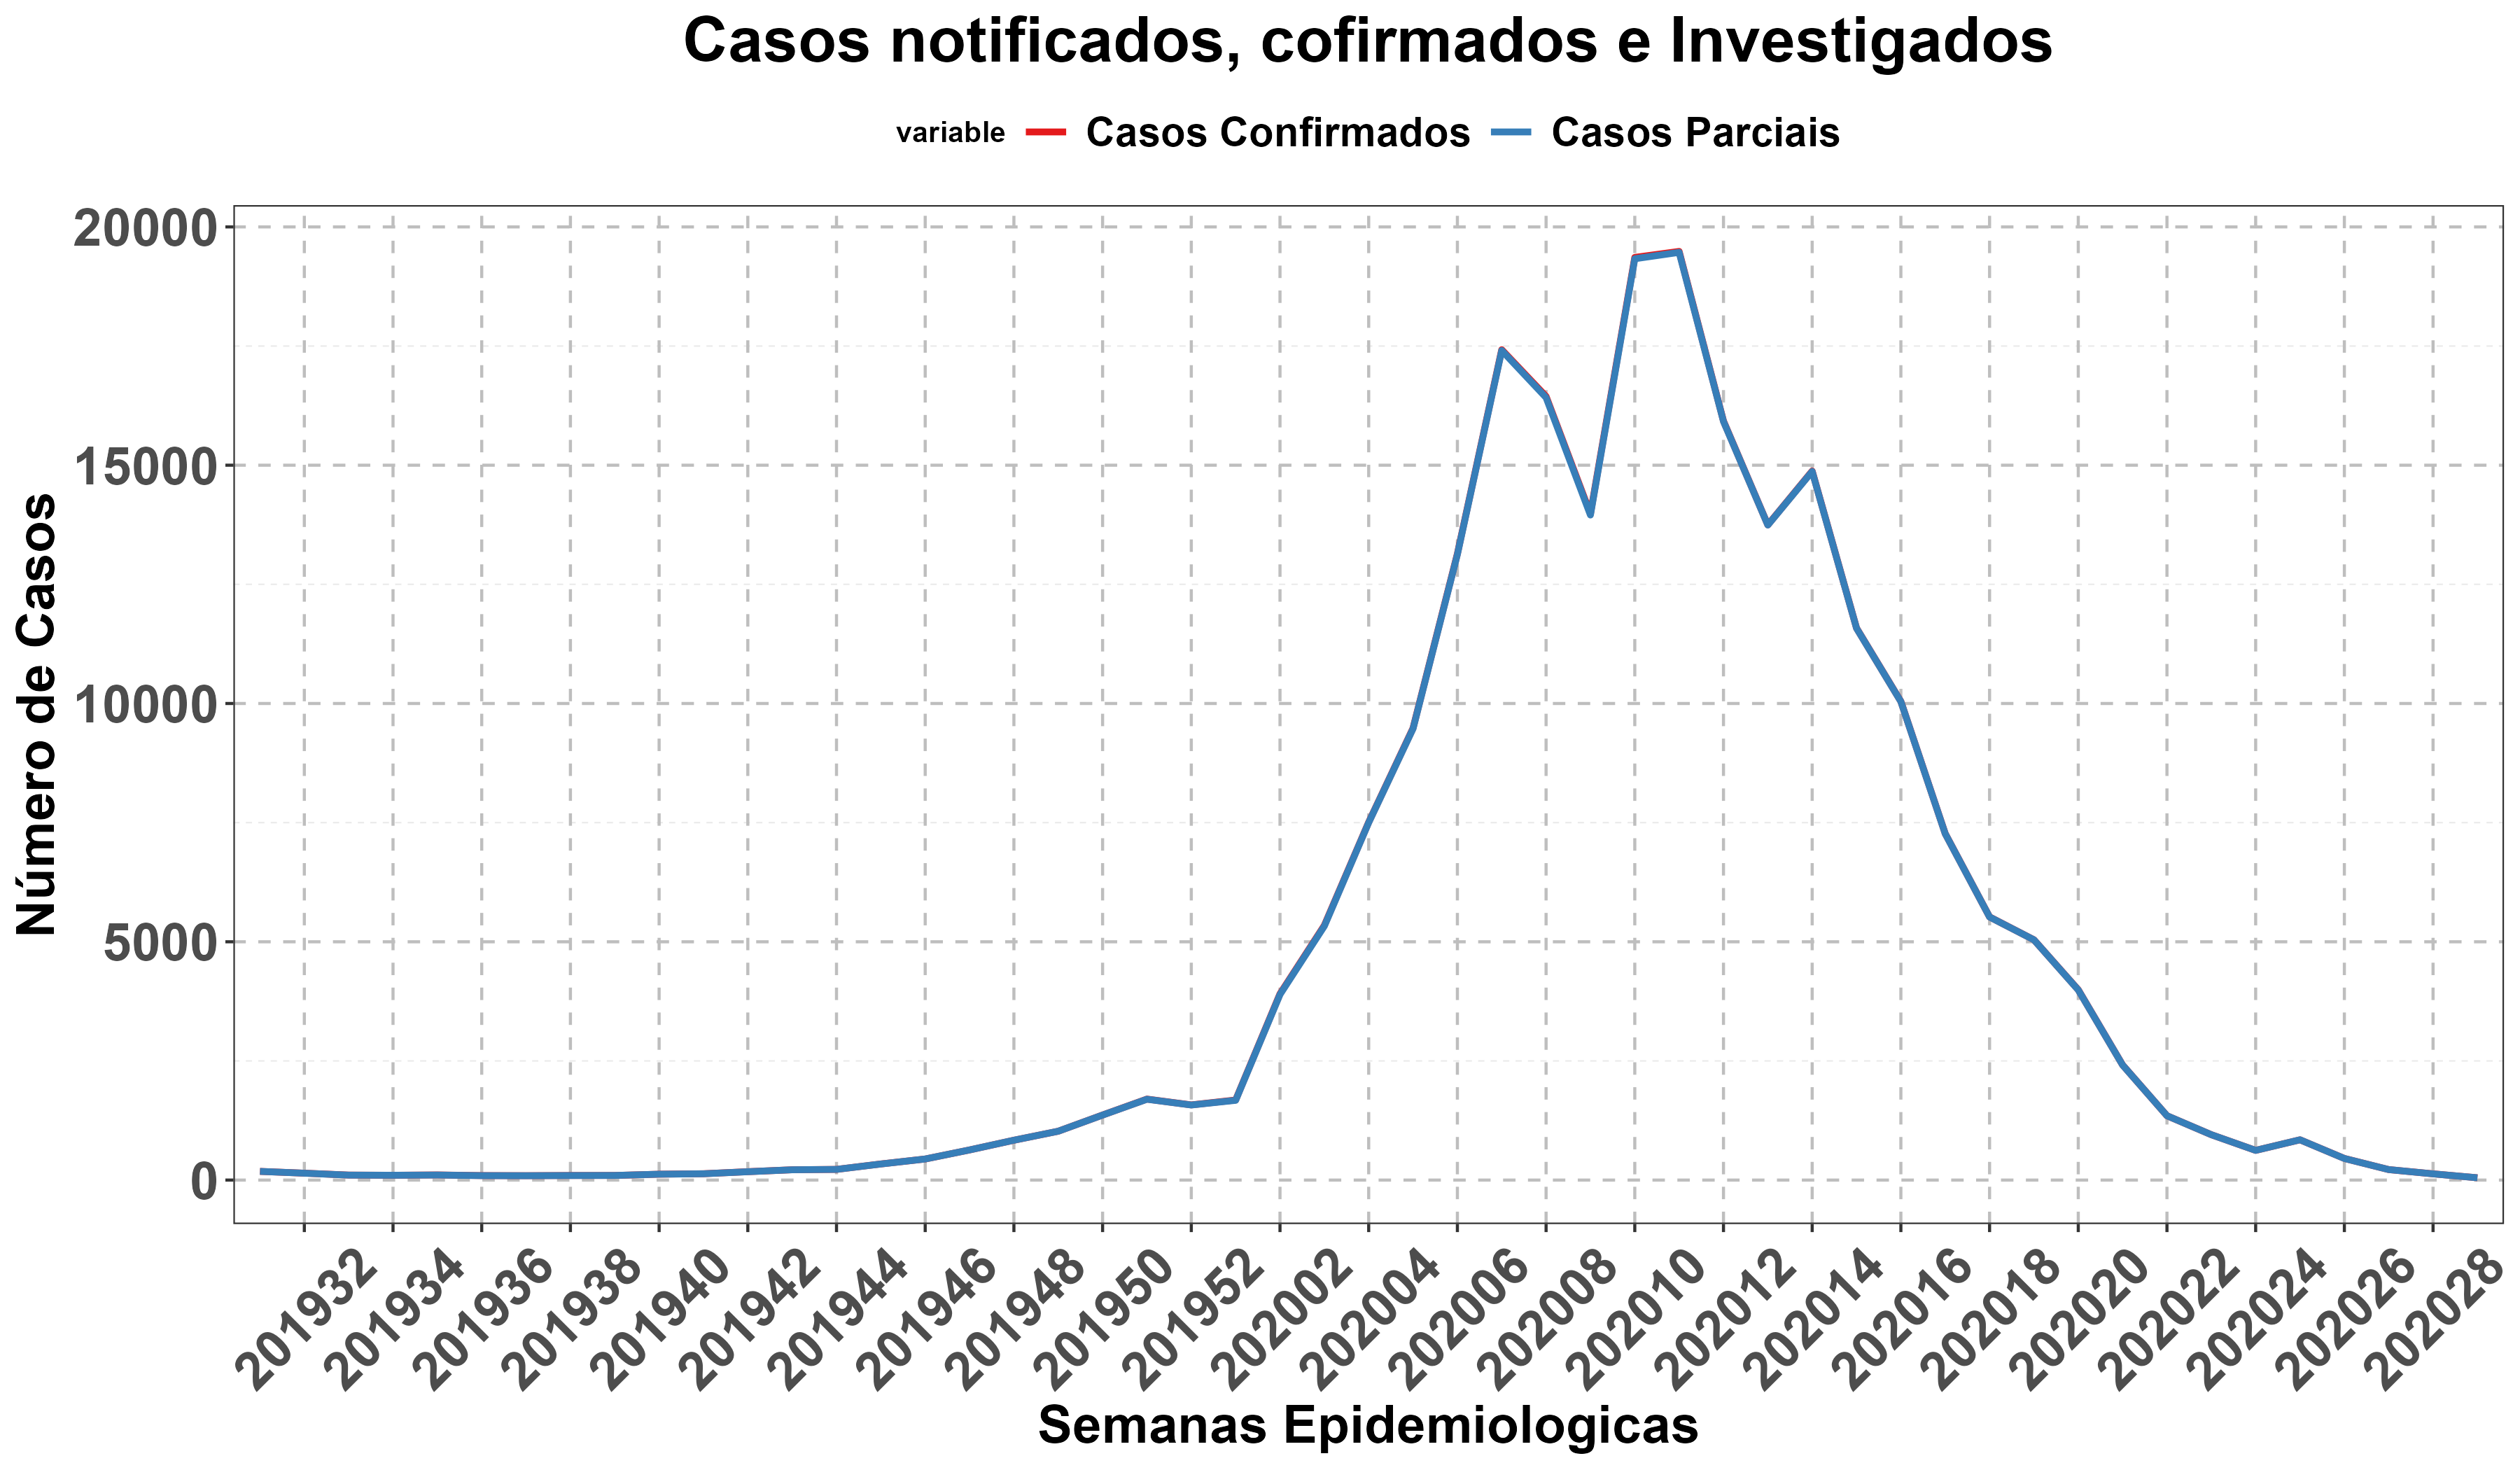
\includegraphics[width=16cm ]{Rplot1.png} 

\clearpage 

  \begin{center} 
 
\includegraphics[width=\textwidth ]{www/h4.png}  

(N de casos autoctones/100.000habitantes. Parana). \end{center} 


\begin{figure}[h] 

         \begin{minipage}[b]{0.5\textwidth} 

         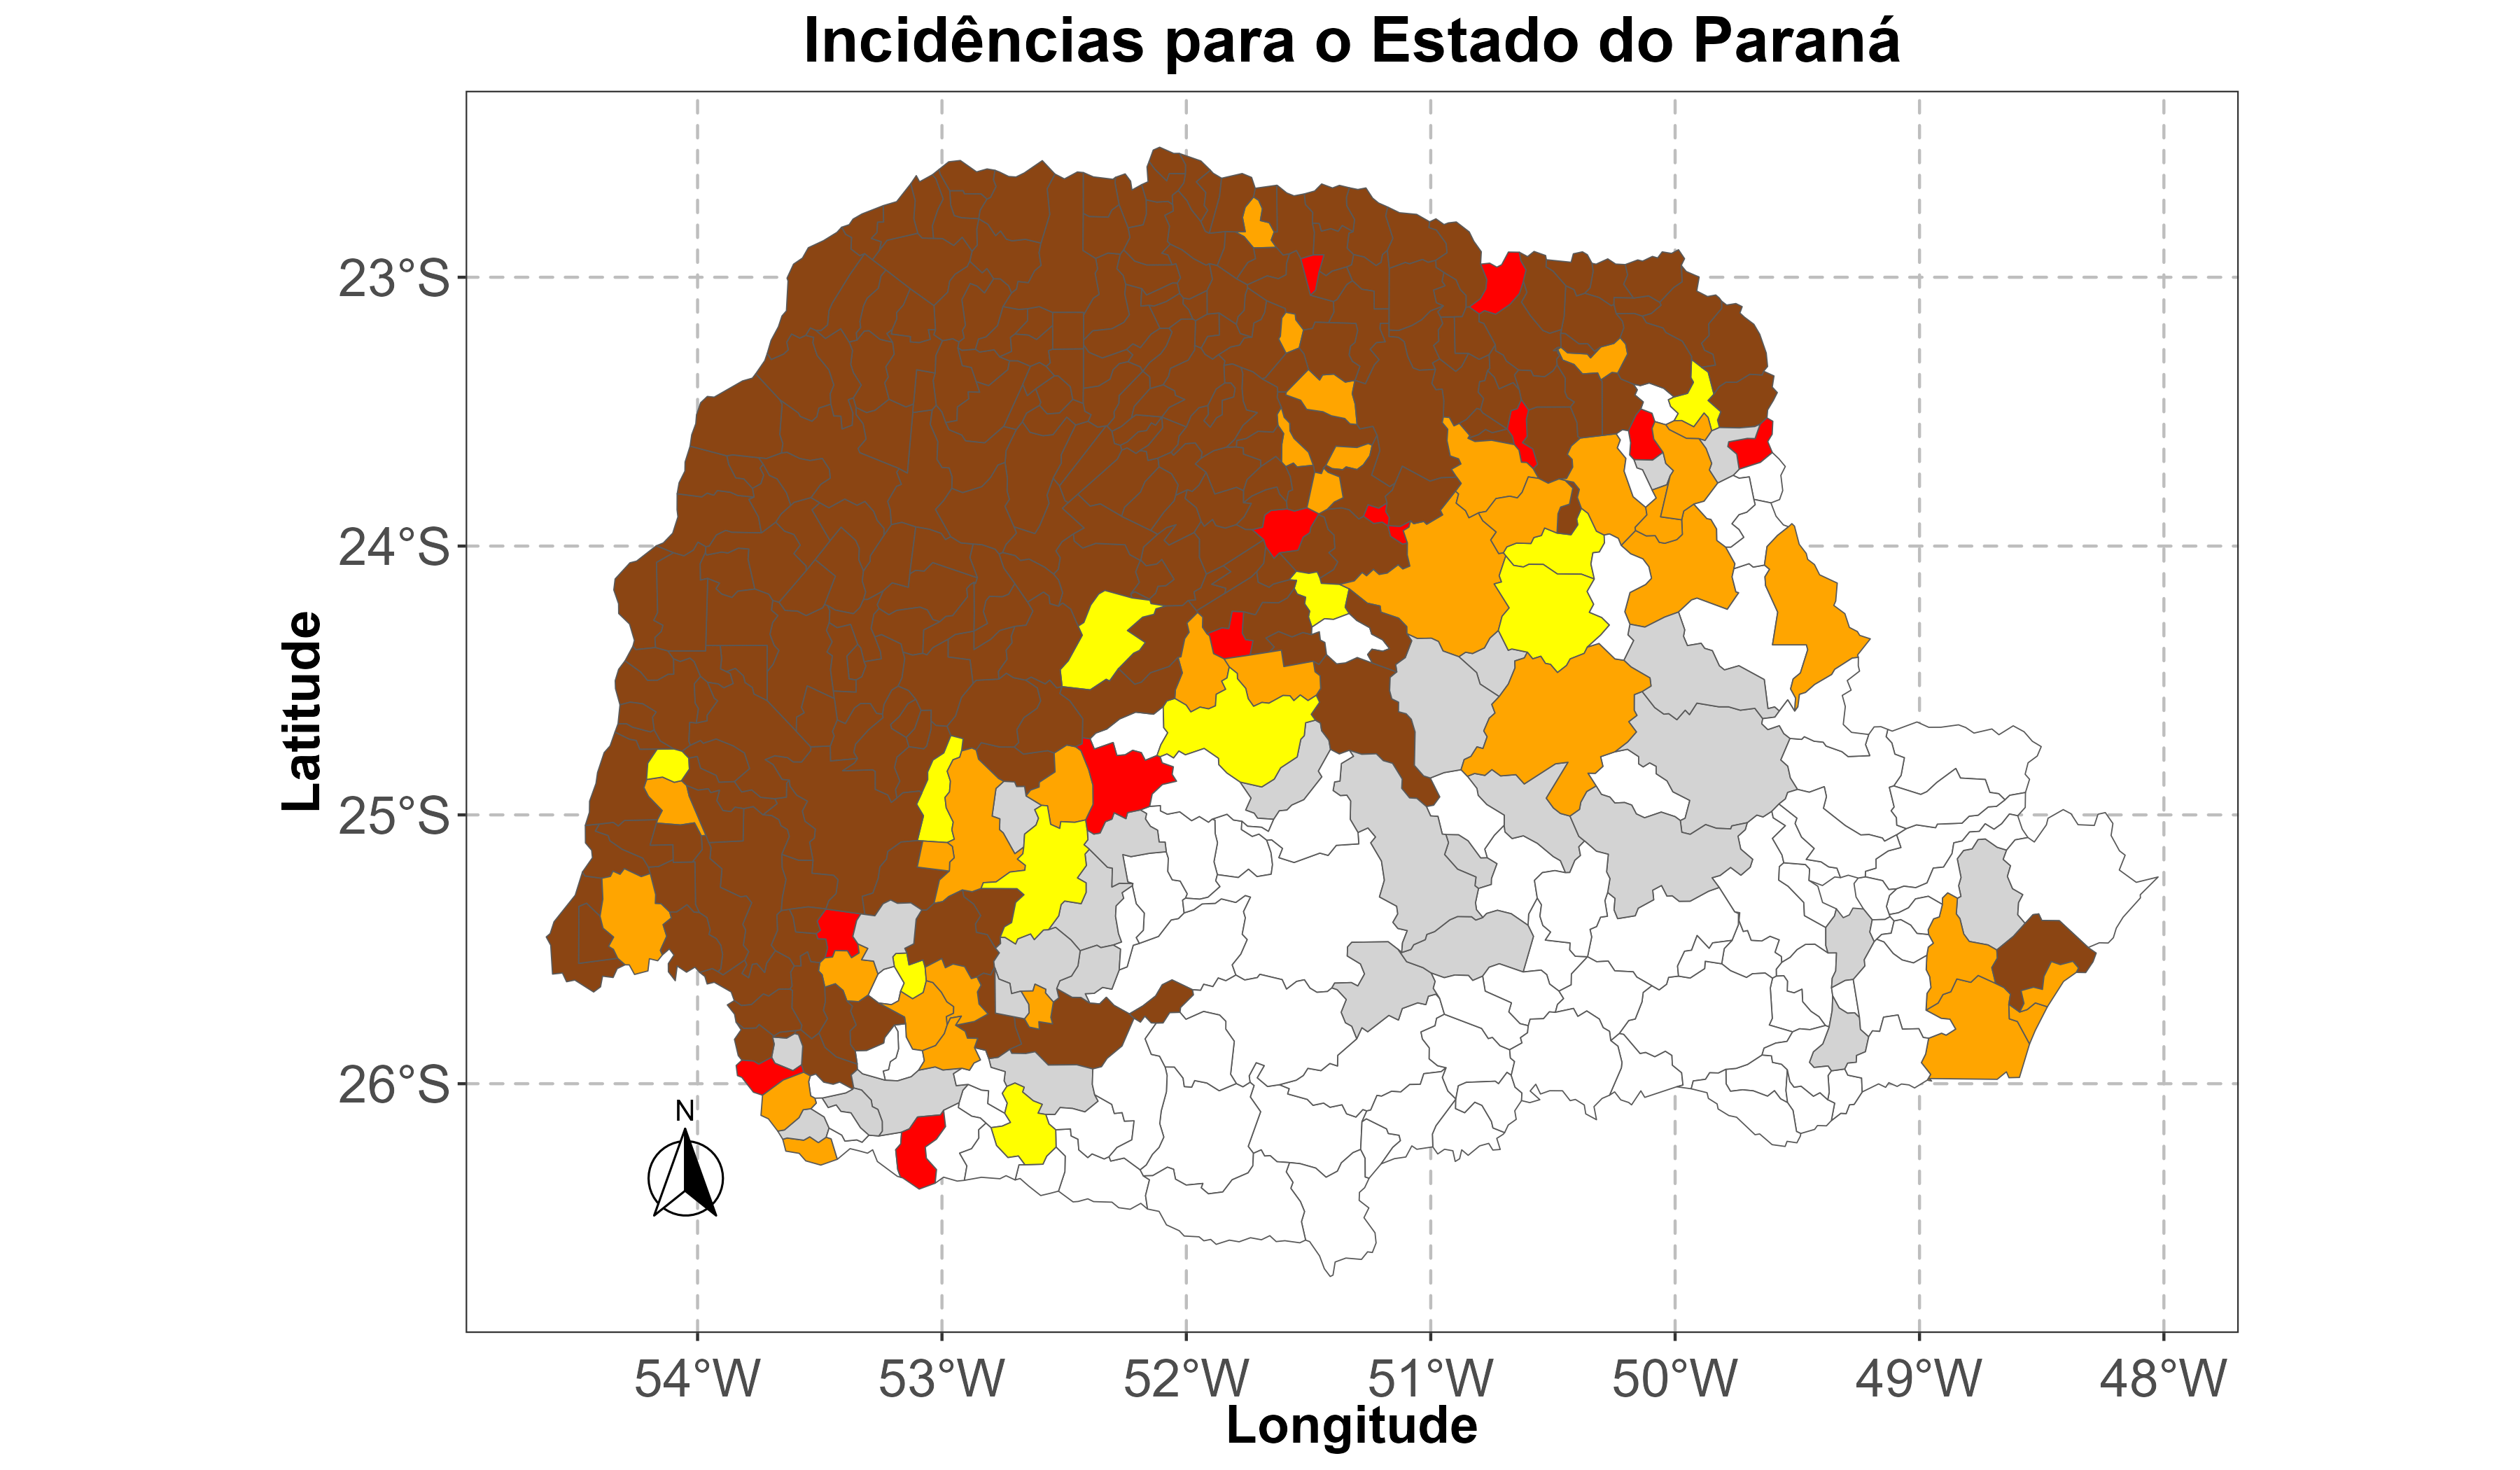
\includegraphics[width=\textwidth]{map_inc.png} 

         \caption{Incidencias para casos autoctonos por 100.000 habitantes} 

         \label{fig:1} 

         \end{minipage} 
         \hfill 
         \begin{minipage}[b]{0.5\textwidth} 

         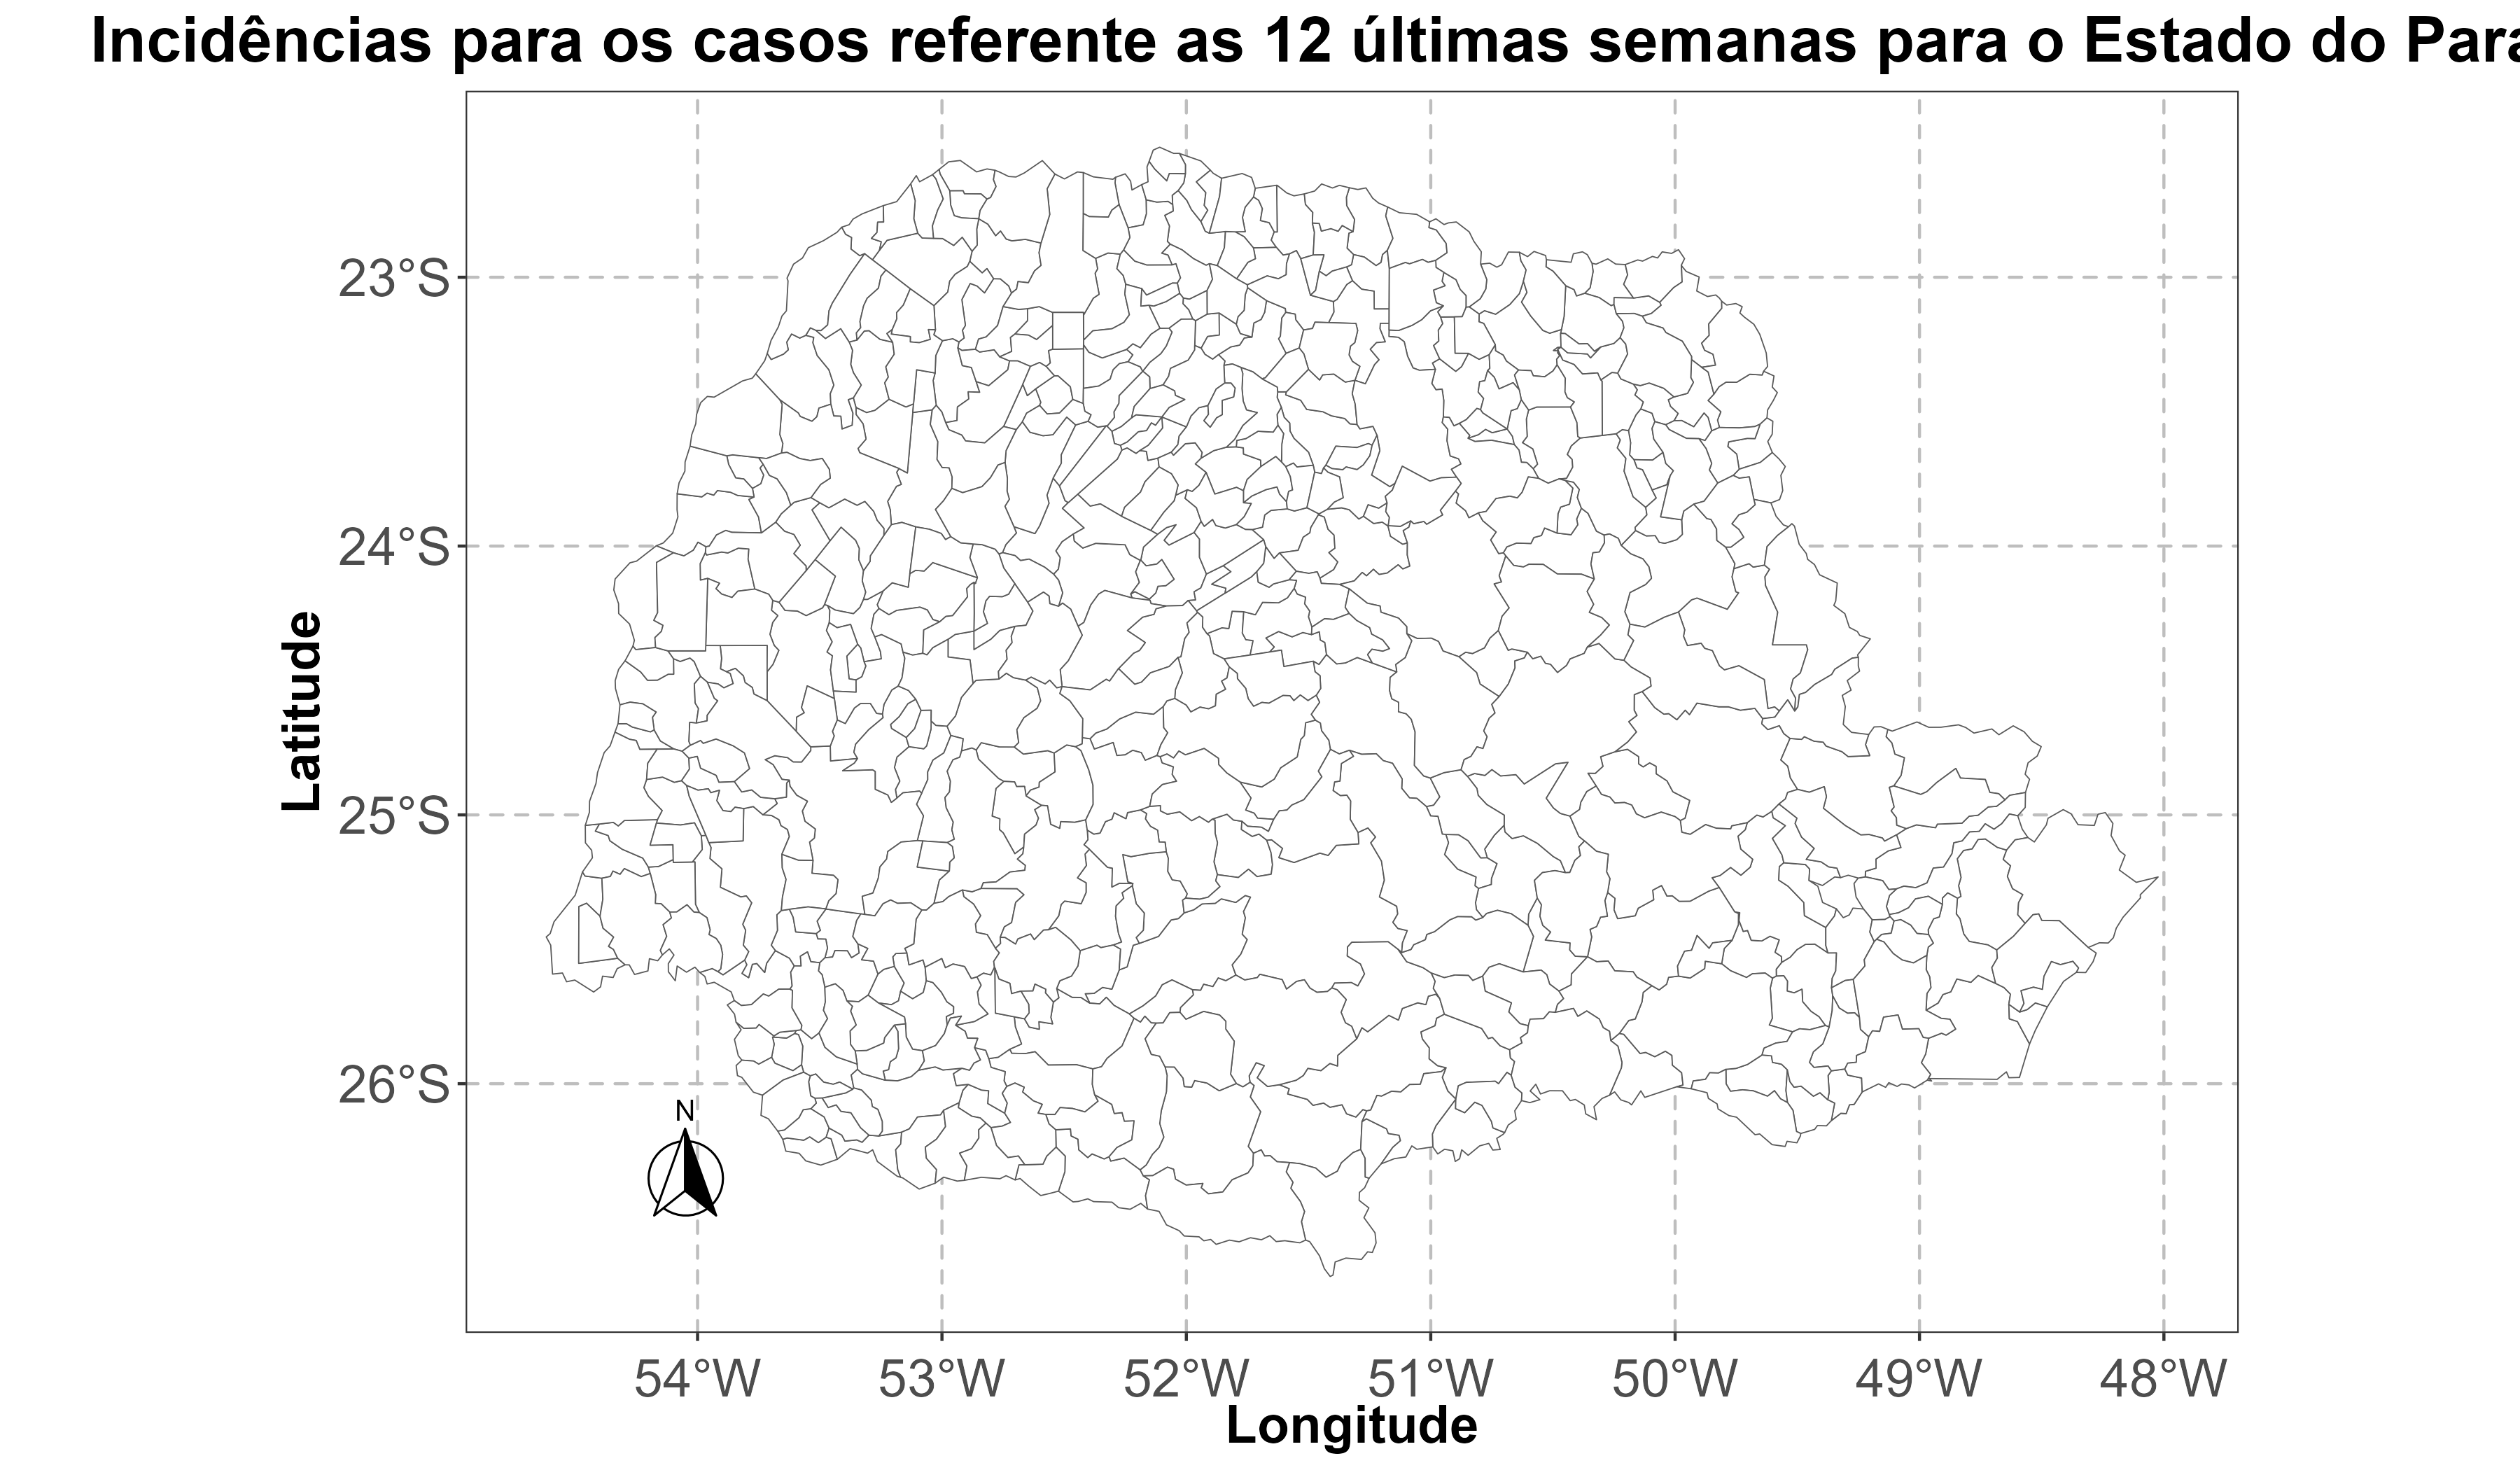
\includegraphics[width=\textwidth]{map_inc4.png} 

         \caption{Incidencias para casos autoctonos por 100.000 habitantes das ultimas 4 semanas.} 

         \label{fig:2} 

         \end{minipage} 

         \end{figure} 
\begin{figure}[h] 

         \begin{minipage}[b]{0.5\textwidth} 

         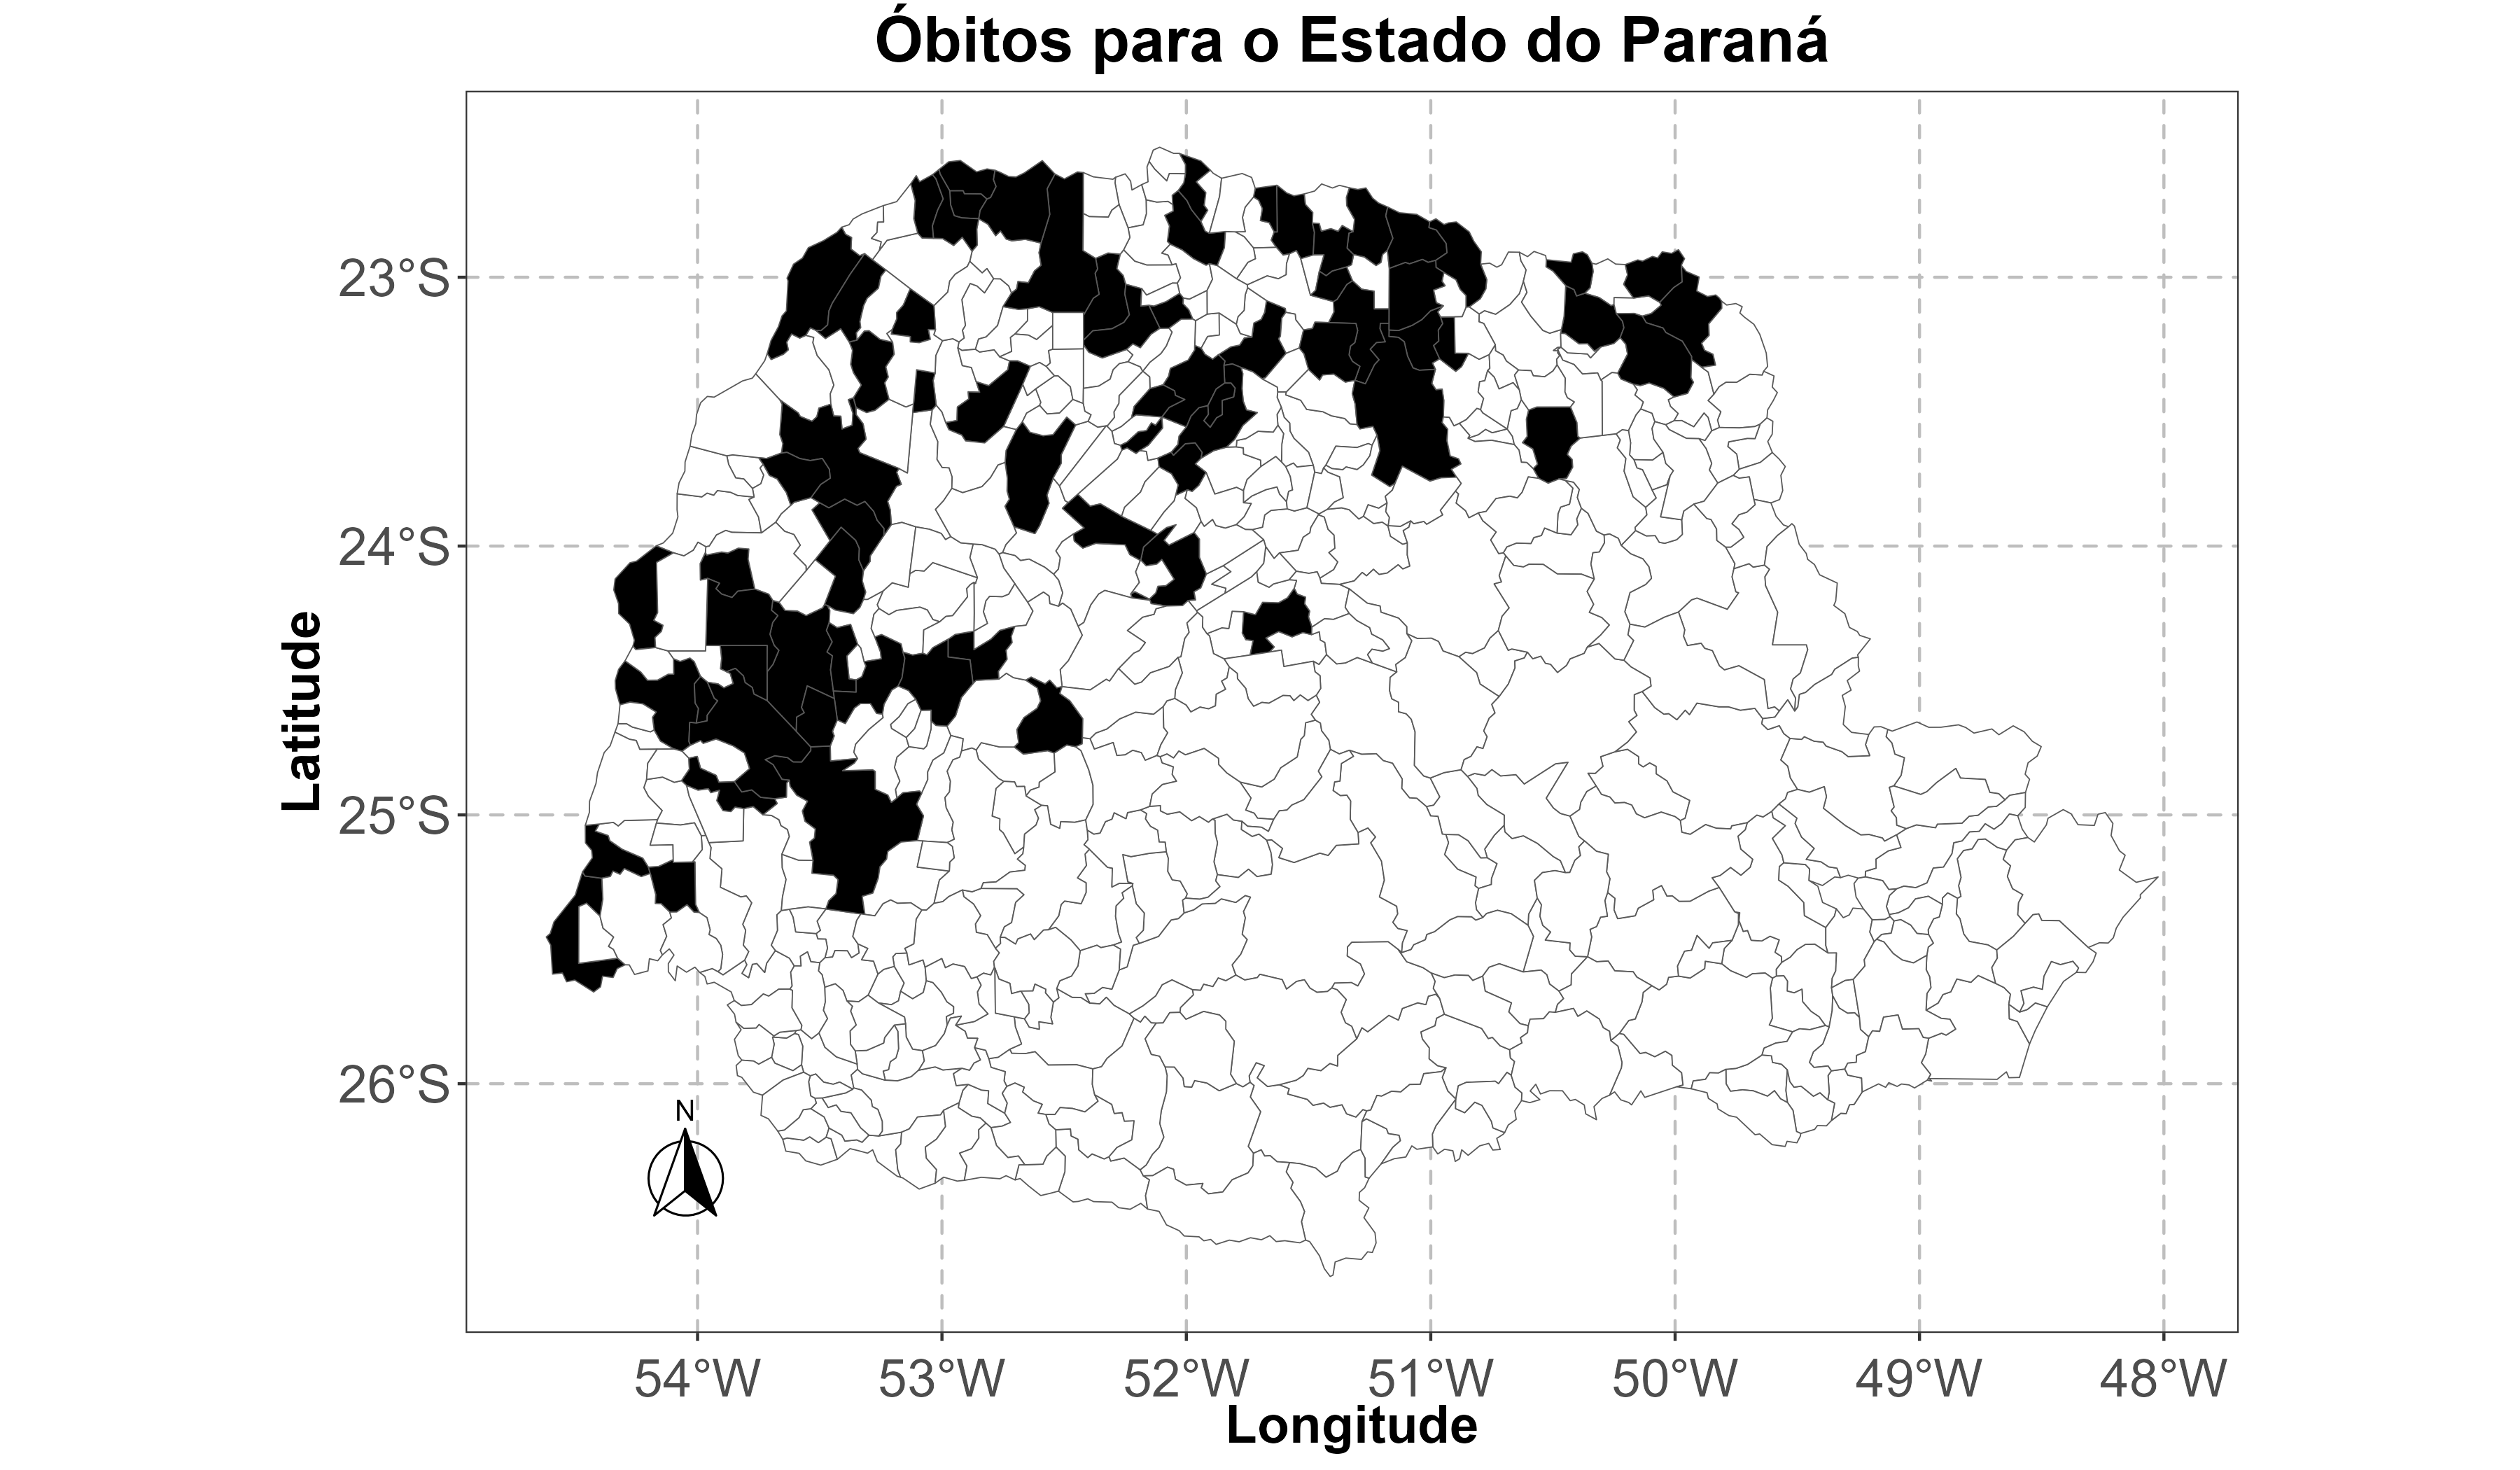
\includegraphics[width=\textwidth]{map_obt.png} 

         \caption{Cidades com Obitos para o Estado do Parana.} 

         \label{fig:1} 

         \end{minipage} 
         \hfill 
         \begin{minipage}[b]{0.5\textwidth} 

         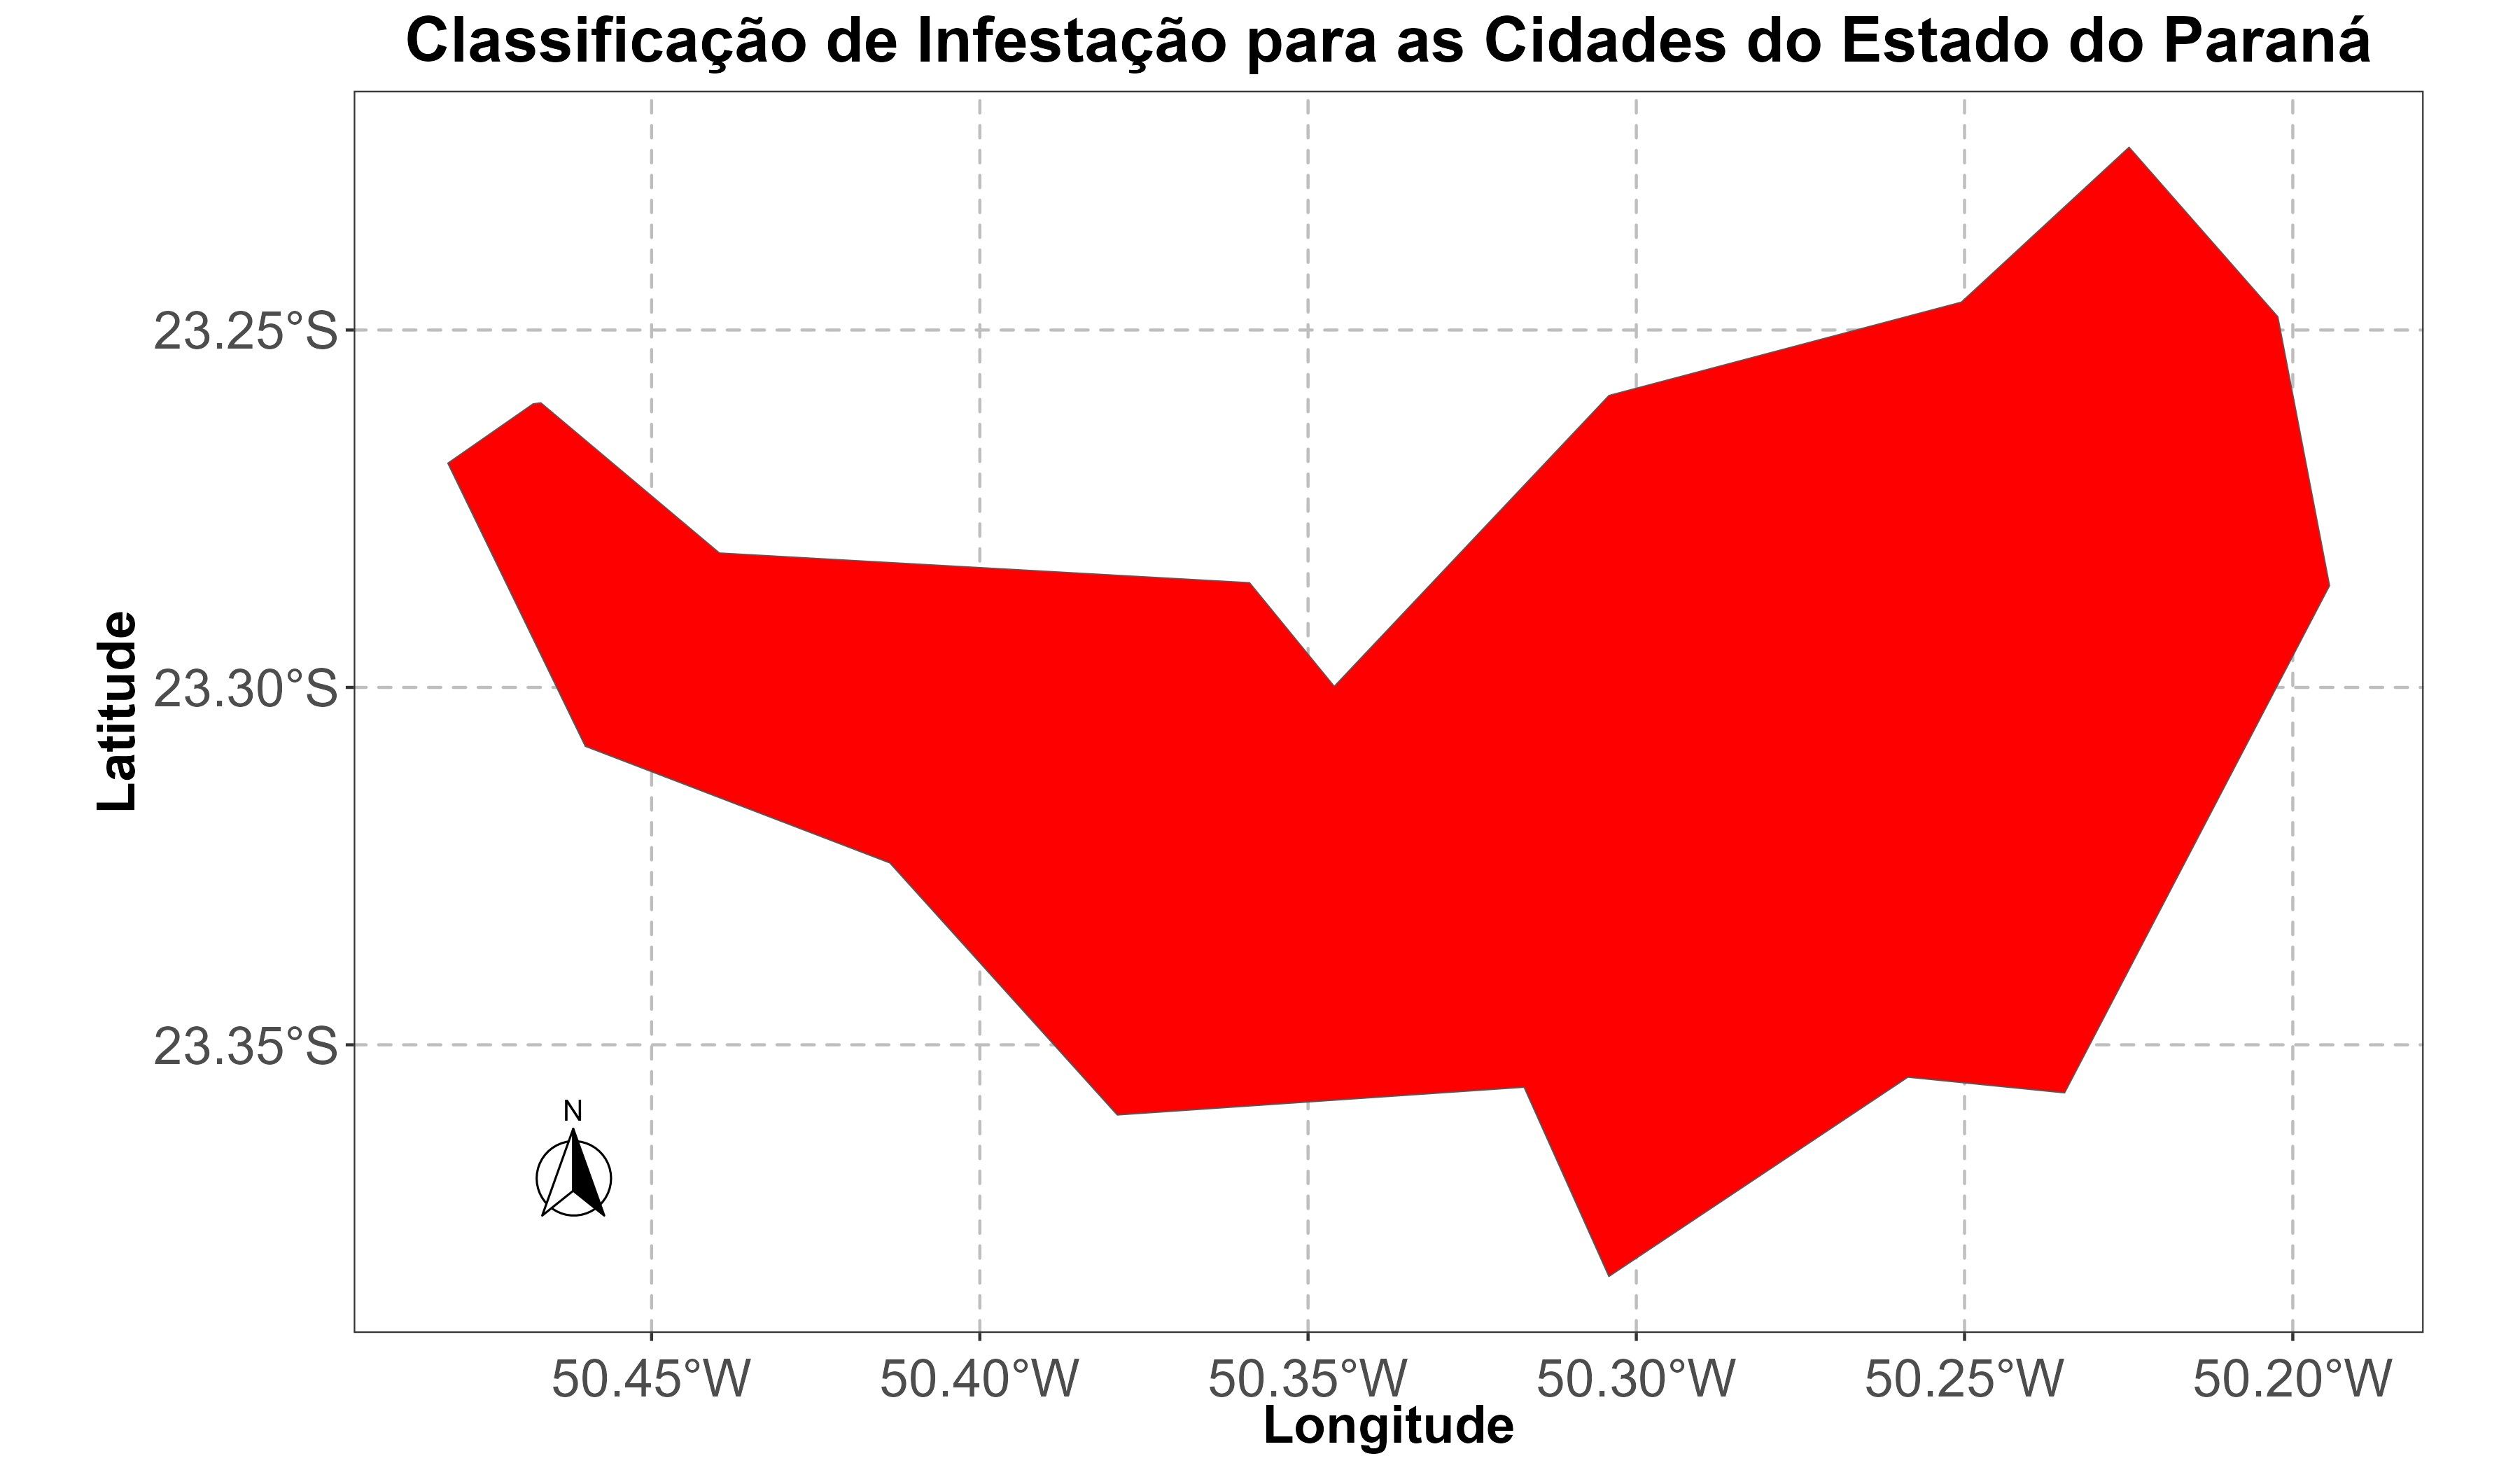
\includegraphics[width=\textwidth]{map_lia.png} 

         \caption{LIA} 

         \label{fig:2} 

         \end{minipage} 

         \end{figure} 
\clearpage 

 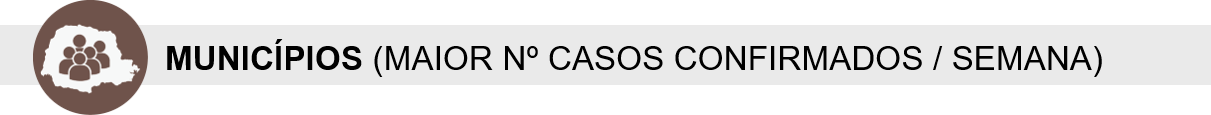
\includegraphics[width=\textwidth ]{www/h5.png}  

\begin{table}[!h]

\caption{Municipios com maior numero de casos das 12 ultimas semanas (> 100)}
\centering
\begin{tabular}[t]{cccc}
\toprule
Macrorregional & Regional de Saude & Municipio & Casos\\
\midrule
Norte & 17 & Londrina & 21575\\
Oeste & 9 & Foz Do Iguacu & 19336\\
Noroeste & 15 & Maringa & 11549\\
Noroeste & 14 & Paranavai & 7601\\
Oeste & 10 & Cascavel & 7518\\
\addlinespace
Norte & 17 & Cambe & 6773\\
Noroeste & 12 & Umuarama & 6371\\
Norte & 17 & Rolandia & 6038\\
Oeste & 20 & Toledo & 4792\\
Norte & 17 & Ibipora & 4666\\
\bottomrule
\end{tabular}
\end{table}\clearpage 

 
\includegraphics[width=\textwidth ]{www/h6.png}  

 \begin{table}[!h]

\caption{Resumo dos casos por Regional de Saude}
\centering
\begin{tabular}[t]{ccccccccc}
\toprule
regional & Macro & Regionais de Saude & Populacao & Casos & DSA & DG & Obitos & Incidencia\\
\midrule
1 & Leste & 1 & 297029 & 2103 & 4 & 1 & 0 & 708.0116756\\
2 & Leste & 2 & 3545708 & 363 & 3 & 1 & 0 & 10.2377297\\
3 & Leste & 3 & 637293 & 145 & 4 & 0 & 0 & 22.7524859\\
4 & Leste & 4 & 174933 & 13 & 1 & 0 & 0 & 7.4314166\\
5 & Leste & 5 & 456587 & 148 & 2 & 0 & 0 & 32.4144139\\
\addlinespace
6 & Leste & 6 & 177311 & 1 & 0 & 0 & 0 & 0.5639808\\
7 & Leste & 7 & 267234 & 425 & 14 & 0 & 0 & 159.0366495\\
8 & Oeste & 8 & 358144 & 2368 & 14 & 1 & 0 & 661.1865618\\
9 & Oeste & 9 & 404414 & 23477 & 474 & 57 & 15 & 5805.1897313\\
10 & Oeste & 10 & 550709 & 17364 & 324 & 7 & 7 & 3153.0263715\\
\addlinespace
11 & Noroeste & 11 & 328863 & 15648 & 116 & 15 & 14 & 4758.2123863\\
12 & Noroeste & 12 & 276371 & 18642 & 136 & 11 & 8 & 6745.2808001\\
13 & Noroeste & 13 & 160642 & 8023 & 25 & 8 & 5 & 4994.3352299\\
14 & Noroeste & 14 & 275974 & 22083 & 185 & 20 & 21 & 8001.8407531\\
15 & Noroeste & 15 & 838017 & 34462 & 259 & 27 & 31 & 4112.3270769\\
\addlinespace
16 & Norte & 16 & 384198 & 2943 & 5 & 0 & 0 & 766.0112754\\
17 & Norte & 17 & 964251 & 48246 & 943 & 102 & 54 & 5003.4690138\\
18 & Norte & 18 & 222583 & 8511 & 52 & 7 & 7 & 3823.7421546\\
19 & Norte & 19 & 289020 & 5157 & 158 & 4 & 4 & 1784.3055844\\
20 & Oeste & 20 & 398323 & 18882 & 113 & 16 & 17 & 4740.3740181\\
\addlinespace
21 & Leste & 21 & 188456 & 198 & 1 & 0 & 0 & 105.0643121\\
22 & Norte & 22 & 128645 & 3156 & 34 & 2 & 1 & 2453.2628551\\
\bottomrule
\end{tabular}
\end{table}\clearpage 

 
\includegraphics[width=\textwidth ]{www/h7.png}  

  
 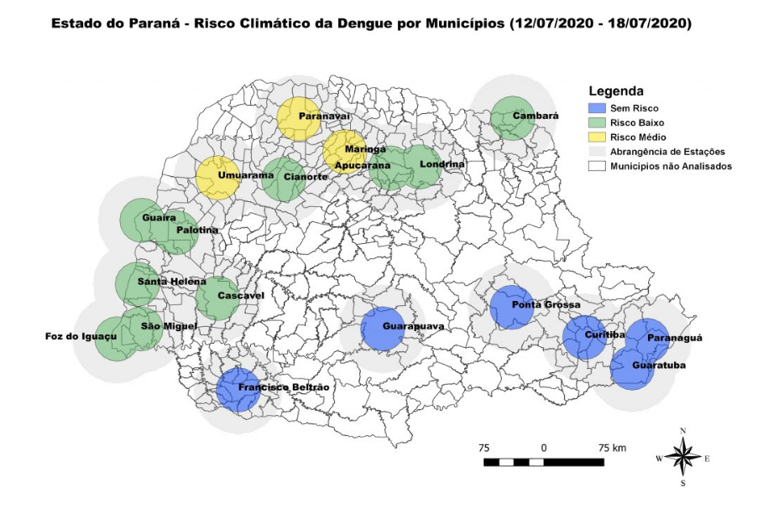
\includegraphics[width=16cm ]{www/risco_climatico.png} 

\clearpage 

 
\includegraphics[width=\textwidth ]{www/h8.png}  

 O quadro abaixo apresenta a série histórica do sorotipo viral de dengue desde o ano de 1991. Observa-se uma predominância do sorotipo DEVN1 até 2018, e do sorotipo DENV2 a partir de 2019.
         De janeiro a 11 de julho de 2020 foram processadas 11.594 amostras para vigilância epidemiológica da circulação viral dos 4 sorotipos. Em 79,7 % das amostras positivas para dengue foi encontrado o sorotipo DENV2.

  
 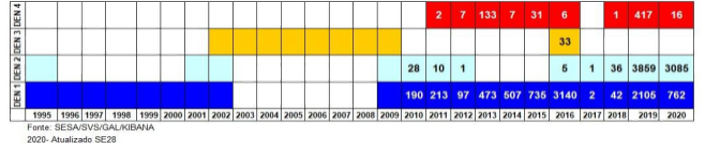
\includegraphics[width=16cm ]{www/quadro_laboratorial.png} 

  
 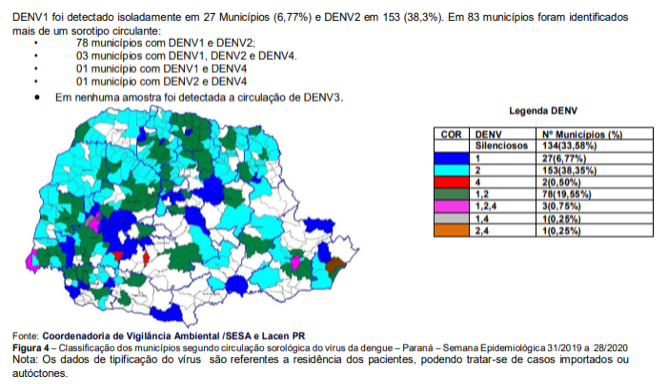
\includegraphics[width=16cm ]{www/mapa_laboratorial.png} 

\clearpage 

  \begin{center} 
 
\includegraphics[width=\textwidth ]{www/header_zika.png} 

   
 
\includegraphics[width=\textwidth ]{www/h2_resumo.png} 
 \end{center} 
 \vspace{-1.5cm} 
  \begin{flushleft} 

              \begin{tabular}{ c c c c c c }
  \hspace{0.5cm} {\Large  364319 } &  \hspace{1.0cm} {\Large  232370 } &  \hspace{1.0cm} {\Large  205033 } &  \hspace{1.0cm} {\Large  1793.194 } &  \hspace{1.1cm} {\Large  382 } &  \hspace{1.8cm} {\Large  184 } \\ 
  \end{tabular}

                 \end{flushleft}


  \begin{center} 
 
\includegraphics[width=\textwidth ]{www/header_chikungunya.png} 

   
 
\includegraphics[width=\textwidth ]{www/h2_resumo.png} 
 \end{center} 
 \vspace{-1.5cm} 
  \begin{flushleft} 

              \begin{tabular}{ c c c c c c }
  \hspace{0.5cm} {\Large  364319 } &  \hspace{1.0cm} {\Large  232370 } &  \hspace{1.0cm} {\Large  205033 } &  \hspace{1.0cm} {\Large  1793.194 } &  \hspace{1.1cm} {\Large  382 } &  \hspace{1.8cm} {\Large  184 } \\ 
  \end{tabular}

                 \end{flushleft}
